\subsubsection{Filtracja chmury punktów}
Ważny i wpływający na jakość wynikowej rekonstrukcji element przetwarzania chmury punktów, jakim jest jej filtracja, pojawia się na dwóch etapach projektu: po przeprowadzeniu generacji chmury punktów i przed uruchomieniem algorytmu segmentacji. 

Celem filtracji, która ma miejsce bezpośrednio po wygenerowaniu chmury punktów, a przed uruchomieniem algorytmu Gaussian Splatting, jest usunięcie szumów. Pozwoli ono na poprawę reprezentacji danych wejściowych do algorytmu oraz na redukcję liczby punktów nieistotnych, co ważne jest w kontekście optymalizacji zapotrzebowania na zasoby obliczeniowe.

Przy implementacji tego elementu wykorzytano funkcjonalność statystycznego usuwania punktów odstających (\textit{ang. statistical outlier removal}) oferowaną przez szeroko stosowaną w przetwarzaniu danych przestrzennych bibliotekę Open3D\cite{Zhou2018}. Metoda ta analizuje lokalną gęstość punktów na podstawie wybranej liczby sąsiadów. Z wykorzystaniem ustalanego progu związanego z odchyleniem standardowym średnich odległości w chmurze punktów odrzucane są punkty, które znajdują się dalej od swoich sąsiadów w porównaniu do średniej dla chmury. 

Filtracja chmury punktów przed segmentacją ma za zadanie eliminować punkty, które znajdują się 
statystycznie dalej od centralnego obszaru chmury, co pozwoli na ograniczenie jej do bardziej zwartej struktury. W ramach tej filtracji zaimplementowano metodę\cite{raviteja2023outliers}, która początkowo określa zakres wyznaczając dla każdej współrzędnej pierwszy kwartyl \textit{Q1}, trzeci kwartyl \textit{Q3} i rozstęp międzykwartylowy $IQR = Q1 - Q3$. Na ich podstawie obliczane są z użyciem parametru $\alpha$ granice zakresu: $Q1 - \alpha * IQR$ i $Q3 + \alpha * IQR$. Odrzucane zostają punkty, dla których wartość którejkolwiek ze współrzędnych znajduje się poza wyznaczonym zakresem.

\begin{figure}[!ht]
  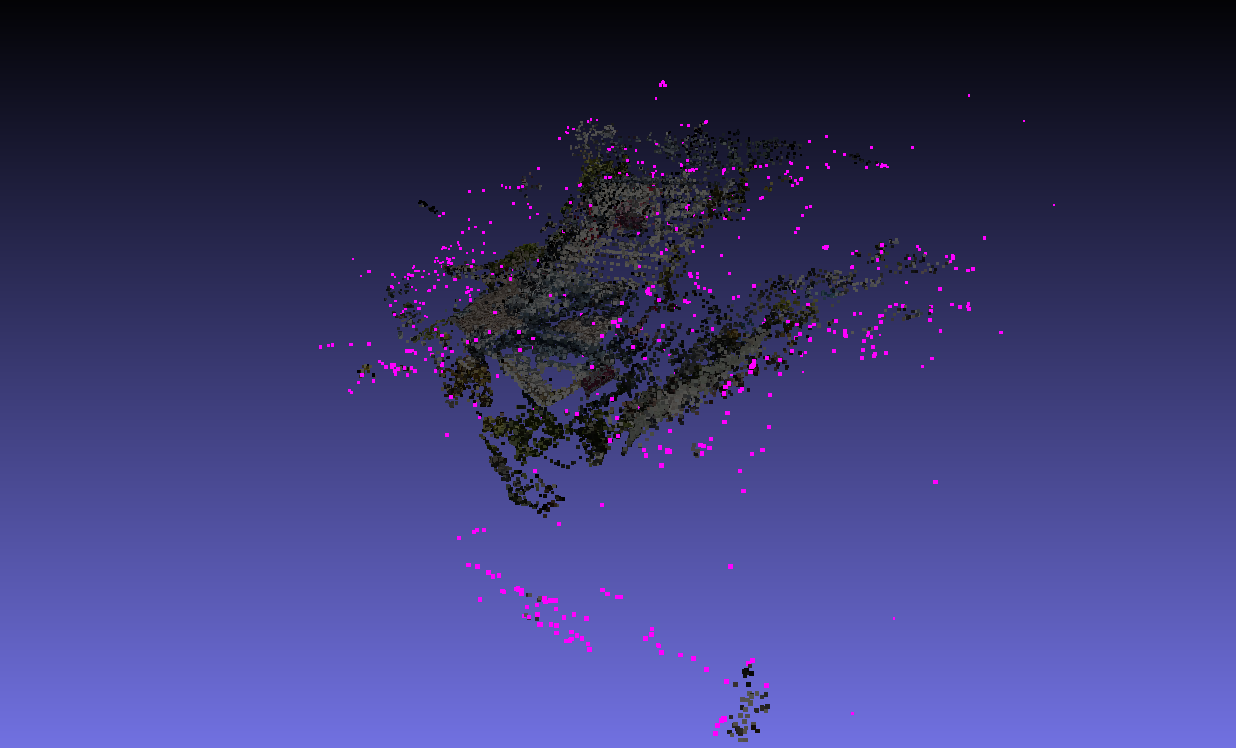
\includegraphics[width=\linewidth]{img/filtering.png}
  \caption{Wizualizacja filtracji chmury punktów, na różowo oznaczono punkty odrzucane}
  \label{fig:filtering}
\end{figure}